\documentclass[]{article}
\usepackage{lmodern}
\usepackage{graphicx}
\usepackage{amssymb,amsmath}
\usepackage{ifxetex,ifluatex}
\usepackage{fixltx2e} % provides \textsubscript
\usepackage{makecell}
\ifnum 0\ifxetex 1\fi\ifluatex 1\fi=0 % if pdftex
  \usepackage[T1]{fontenc}
  \usepackage[utf8]{inputenc}
\else % if luatex or xelatex
  \ifxetex
    \usepackage{mathspec}
  \else
    \usepackage{fontspec}
  \fi
  \defaultfontfeatures{Ligatures=TeX,Scale=MatchLowercase}
\fi
% use upquote if available, for straight quotes in verbatim environments
\IfFileExists{upquote.sty}{\usepackage{upquote}}{}
% use microtype if available
\IfFileExists{microtype.sty}{%
\usepackage[]{microtype}
\UseMicrotypeSet[protrusion]{basicmath} % disable protrusion for tt fonts
}{}
\PassOptionsToPackage{hyphens}{url} % url is loaded by hyperref
\usepackage[unicode=true]{hyperref}
\hypersetup{
            pdftitle={Specyfikacja implementacyjna programu realizującego dekompresję plików skompresowanych algorytmem Huffmana},
            pdfauthor={Adrian Chmiel, Mateusz Tyl},
            pdfborder={0 0 0},
            breaklinks=true}
\urlstyle{same}  % don't use monospace font for urls
\IfFileExists{parskip.sty}{%
\usepackage{parskip}
}{% else
\setlength{\parindent}{0pt}
\setlength{\parskip}{6pt plus 2pt minus 1pt}
}
\setlength{\emergencystretch}{3em}  % prevent overfull lines
\providecommand{\tightlist}{%
  \setlength{\itemsep}{0pt}\setlength{\parskip}{0pt}}
\setcounter{secnumdepth}{0}
% Redefines (sub)paragraphs to behave more like sections
\ifx\paragraph\undefined\else
\let\oldparagraph\paragraph
\renewcommand{\paragraph}[1]{\oldparagraph{#1}\mbox{}}
\fi
\ifx\subparagraph\undefined\else
\let\oldsubparagraph\subparagraph
\renewcommand{\subparagraph}[1]{\oldsubparagraph{#1}\mbox{}}
\fi

% set default figure placement to htbp
\makeatletter
\def\fps@figure{htbp}
\makeatother


\title{Specyfikacja implementacyjna programu realizującego dekompresję plików skompresowanych algorytmem Huffmana}
\author{Autorzy: Adrian Chmiel, Mateusz Tyl}
\date{10.06.2023}



\begin{document}
\maketitle
\begin{center}
Historia zmian dokumentu:\\
\end{center}

\begin{tabular}{|c|c|c|c|}
  \hline 
  Autor: & Data: & Opis zmiany:& Wersja dokumentu \\
  \hline
  Adrian Chmiel & 10.06.2023 & Pierwsza wersja dokumentu & 1.0 \\
  \hline
  Adrian Chmiel & 10.06.2023 & Drobne poprawki & 1.1 \\
  \hline
  Adrian Chmiel & 10.06.2023 & Dodanie schematów klas & 2.0 \\
  \hline
  Adrian Chmiel & 11.06.2023 & Finalna wersja dokumentu & 3.0 \\
\hline
\end{tabular} 
\section{Cel dokumentu}\label{header-n231}

Celem tego dokumentu jest przedstawienie informacji o sposobie działania programu od strony technicznej poprzez analizę każdego pliku z osobna oraz przedstawienie związków między nimi.
\section{Informacje ogólne}\label{header-n231}
Program realizuje dekompresję plików pochodzących z kompresora przygotowanego w ramach poprzedniego projektu. Został on w całości napisany w języku Java. Dla prawidłowego działania wszystkich komponentów programu zalecane jest korzystanie z wersji JDK 20 lub wyższej.\\
Program jest przystosowany do pracy i kompilacji zarówno na systemach Unixowych, jak i systemie Microsoft Windows. Do dyspozycji programisty przygotowano szeroki zakres testów różnej złożoności do wykonania..

\section{Omówienie kodu źródłowego}\label{header-n231}
Program oferuje kilka modułów, które wzajemnie współpracują ze sobą. Niektóre z nich pracują jednak niezależnie od innych.

\begin{itemize}
\section{Katalog główny}\label{header-n231}
\item Dekompresor.jar -> archiwum zawierające wszystkie klasy znajdujące się w package \textit{dekompresor}
\item README.md -> plik zawierający informacje o projekcie przygotowany pod repozytorium na GitHubie
\section{Package "dekompresor"}\label{header-n231}
\item[]
Zawiera on kod źródłowy klas, które składają się potem na archiwum \textit{Dekompresor.jar}
\item
BitsAnalyze -> zawiera funkcje służące do analizy kolejnych bitów zawartych w kolejnych znakach przy dekompresji oraz analizuje zapisany słownik w pliku. Funkcje korzystają z pomocniczej klasy DNode odwzorowującej drzewo binarne. Zawarte są w niej następujące tryby działania (opisane przy pomocy komentarzy w kodzie): dictRoad - tryb uaktywnia się, gdy przemieszczamy się w drzewie, dictWord - uaktywniany, gdy znajdziemy się w liściu w celu odczytania znaku/słowa, bitsToWords - służy do odczytywania skompresowanych danych po odczytaniu całości słownika
\item 
Buffer -> klasa zawierająca pomocnicze pola pod tworzenie róznego rodzaju buforów
\item
Controller -> klasa sprawdzająca argumenty podane na wejściu oraz poprawność podanych plików
\item
Decompressor -> klasa zawierająca główne funkcje dekompresujące, które wywołują inne metody pomocnicze oraz zapisują do pliku wyjściowego odczytane znaki
\item
Decrypt -> klasa wykonująca proste odszyfrowanie dla plików zaszyfrowanych i nieskompresowanych
\item
DNode -> klasa tworząca pomocnicze drzewo służące do prawidłowego odczytywania słownika podczas dekompresji
\item
FileManager -> klasa abstrakcyjna wspierająca prawidłowe zarządzanie oraz przygotowywanie plików
\item
Flags -> klasa pomocnicza służąca do sprawnego odczytania flag dla danego pliku
\item
Main -> uruchamia cały proces dekompresji
\item
Mode -> klasa pomocnicza służąca do przechowywania aktualnego trybu
\item
SendDataToGUI -> klasa zawierająca metodę odpowiadającą za uzupełnianie pliku \textit{data} odpowiednimi wartościami, które są następnie pobierane przez GUI
\item
Settings -> klasa pomocnicza służąca do przechowywania wybranych przez użytkownika ustawień przekazanych w argumentach
\item
Utils -> klasa zawierająca pomocnicze metody do sprawdzania poprawności pliku oraz wyświetlania pomocy programu na standardowy strumień
\section{Package "dekompresorgui"}\label{header-n231}
\item[]
W tej części zawarty jest opis klas odpowiadający za graficzne przedstawienie okienka oraz ewentualnej wizualizacji słownika zrealizowany przy pomocy JavaFX.
\item
AnalyzeDataFromDecompressor -> klasa analizująca plik \textit{data} tworzony w trakcie działania programu
\item
CLine -> klasa tworząca linię o określonych parametrach między podanymi koordynatami (w przypadku tego programu dwa środki kwadratów tj. węzłów)
\item
CObject -> interface implementowany przez CLine oraz CRect
\item
CRect -> klasa tworząca kwadrat o określonych parametrach będący danym węzłem w drzewie, w przypadku liścia zawiera również literkę odpowiadającą danemu kodowi
\item
CTree -> klasa realizująca obrazowanie słownika w sposób podobny do wspomnianego wcześniej DNode
\item
DekompresorGUI -> klasa tworząca główne okienko umożliwiające wybór pliku, ustawień itd.
\item
DictTree -> klasa tworząca okienko z wizualizacją całego słownika
\section{Dodatkowe pliki tworzone w trakcie działania programu}\label{header-n231}
\item
data -> plik pomocniczy służący do komunikacji dekompresora z graficznym okienkiem
\item
tree -> plik pomocniczy przechowujący informacje o tym, jak tworzyć drzewo
\end{itemize}

System tworzenia drzewa jest bardzo podobny do systemu zapisu słownika wyjaśnionego w specyfikacji funkcjonalnej, lecz zamiast pojedynczych bitów 00, 01, 10, 11 odpowiednio zapisuję pojedyncze bajty znakami '0', '1', '2', '3'. Sama wizualizacja jest wyświetlania jedynie dla plików skompresowanych 8-bitowo, a więc informacje zawarte w samym pliku \textit{tree} są akuratne również tylko i wyłącznie dla takiej kompresji.

\section{Schemat klas dekompresora}\label{header-n231}
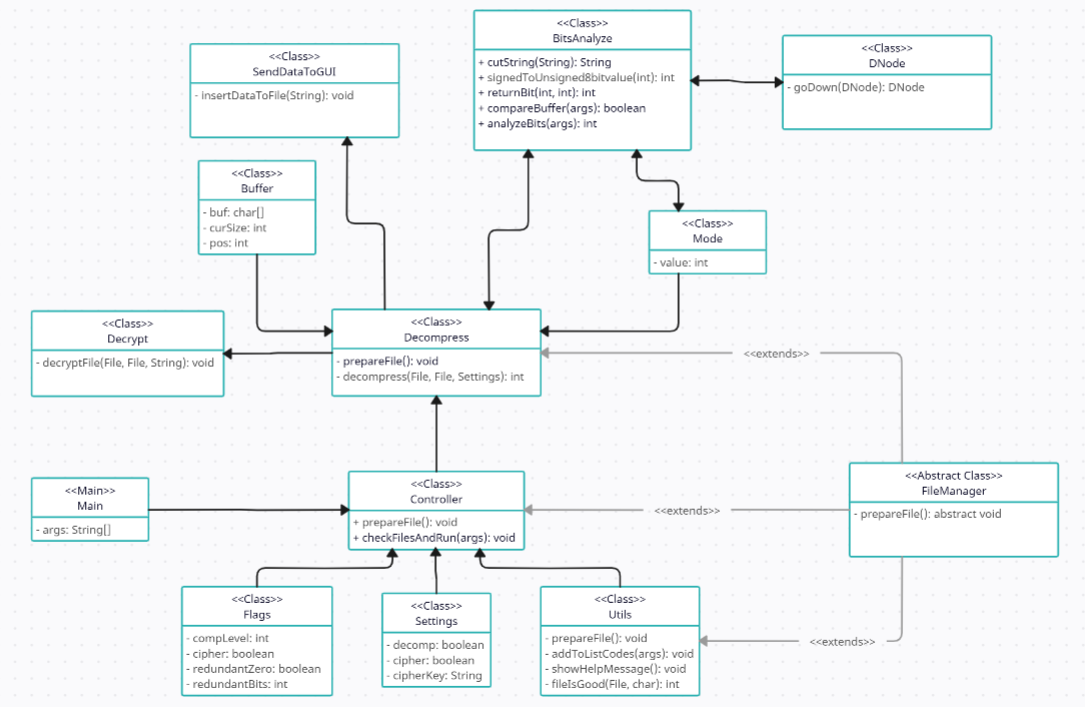
\includegraphics[width=\textwidth]{classes1.png}

\section{Schemat klas odpowiadających za część graficzną}\label{header-n231}
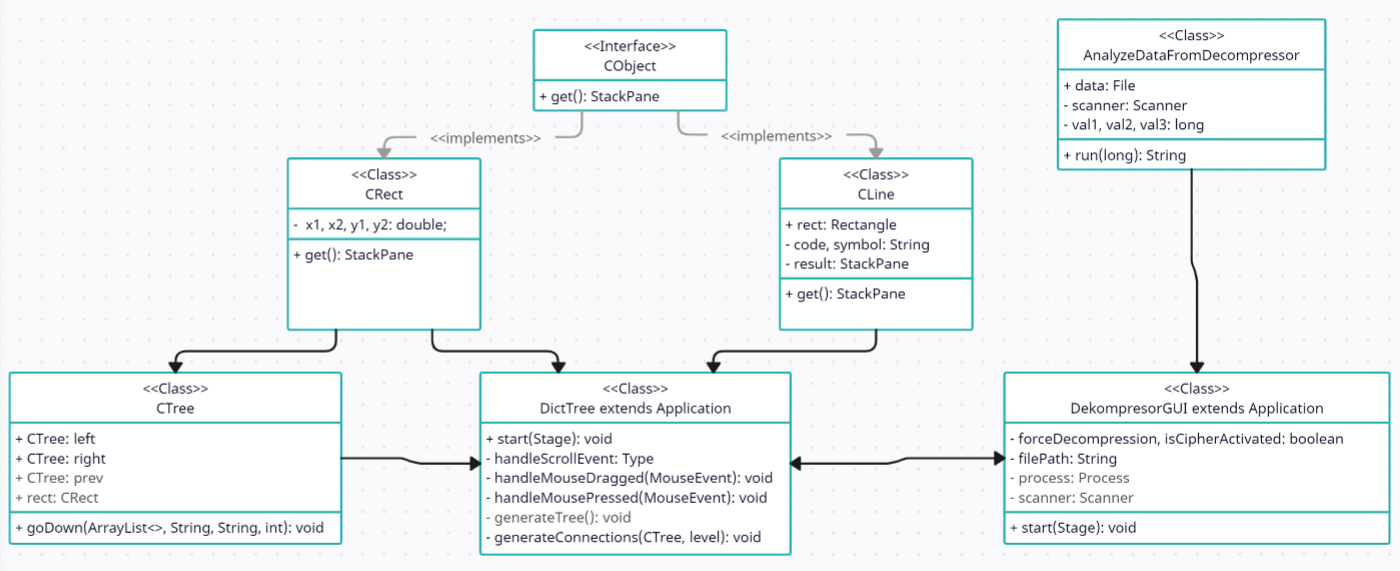
\includegraphics[width=\textwidth]{classes2.png}
\end{document}